\documentclass[dvipdfmx]{beamer}
\usetheme[secheader]{Boadilla}
% \usepackage{beamerthemesplit} // Activate for custom appearanced
%\setbeamertemplate{caption}[numbered]
\usefonttheme[onlymath]{serif} %数式をゴシックにしない
\setbeamertemplate{blocks}[rounded] % Blockの影を消す
\useinnertheme{circles} % 箇条書きをシンプルに
\setbeamertemplate{navigation symbols}{} % ナビゲーションシンボルを消す
\setbeamertemplate{footline}[frame number] % フッターはスライド番号のみ
\setbeamercolor{page number in head/foot}{fg=black}
% \usepackage{beamerthemesplit} // Activate for custom appearance
\setlength{\parindent}{1em}  %段落字下げ
\renewcommand{\figurename}{Fig}
\renewcommand{\tablename}{Tab}
\usepackage{tikz}  
\usetikzlibrary{decorations.pathreplacing,calligraphy}
\setbeamerfont{itemize/enumerate subbody}{size=\normalsize}
%\setbeamertemplate{itemize subitem}{\normalsize\raise1.25pt\hbox{\donotcoloroutermaths$\blacktriangleright$}}  %to set the symbol size
\usepackage{tikz}
\usetikzlibrary{shapes,positioning}

\title{テンソル同時分解の拡張による\\オミクスデータの統合}
\date{2023年6月3日}
\author {阿部興\footnote{東京医科歯科大学難治疾患研究所} ・島村徹平\footnote{名古屋大学医学系研究科・東京医科歯科大学難治疾患研究所}}

\begin{document}
\frame{
\titlepage
}

\renewcommand*{\thefootnote}{\fnsymbol{footnote}}
\setcounter{footnote}{0} 

\section{背景}
\frame{
\frametitle{動機:分析対象}
\begin{figure}
 \begin{tikzpicture}
\node[draw, rounded corners, fill=gray!10](dna) at (0,0){DNA};
\node[draw, rounded corners, fill=gray!10, right = of dna, xshift = +15pt](rna){RNA};
\node[draw, rounded corners, fill=gray!10, right = of rna, xshift = +15pt](protein) {protein};
\node[draw, rounded corners, fill=gray!10, right = of protein](phenotype) {phenotype};
%path
\path[draw, ->, olive](dna)--(rna) node[midway, below, yshift = -2pt]{転写};
\path[draw, ->, olive](rna)--(protein) node[midway, below, yshift = -2pt]{翻訳};
\path[draw, dashed, ->, olive](protein)--(phenotype);
%omics
\node[below= of dna](genomics){genomics};
\node[below= of rna](transcriptomics){transcriptomics};
\node[below= of protein](proteomics){proteomics};

\path[draw, teal](dna)--(genomics);
\path[draw, teal](rna)--(transcriptomics);
\path[draw, teal](proteomics)--(protein);

\path[draw, teal, dashed](genomics.north west)--(proteomics.north east);
\path[draw, teal, dashed](genomics.south west)--(proteomics.south east);
\path[draw, teal, dashed](genomics.north west)--(genomics.south west);
\path[draw, teal, dashed](proteomics.north east)--(proteomics.south east)node[right](omics){-omics};
\end{tikzpicture}
\end{figure}
\begin{itemize}
\item オミクス(-omics)データを統合して分析したい
\begin{itemize}
\item \structure{積極的理由:}データを補い合い普遍的な特徴を抽出
\item \structure{消極的理由:}対応のあるサンプルなので非独立
\end{itemize}
\end{itemize}
}
\frame{
\frametitle{動機:分析手法}
\begin{figure}
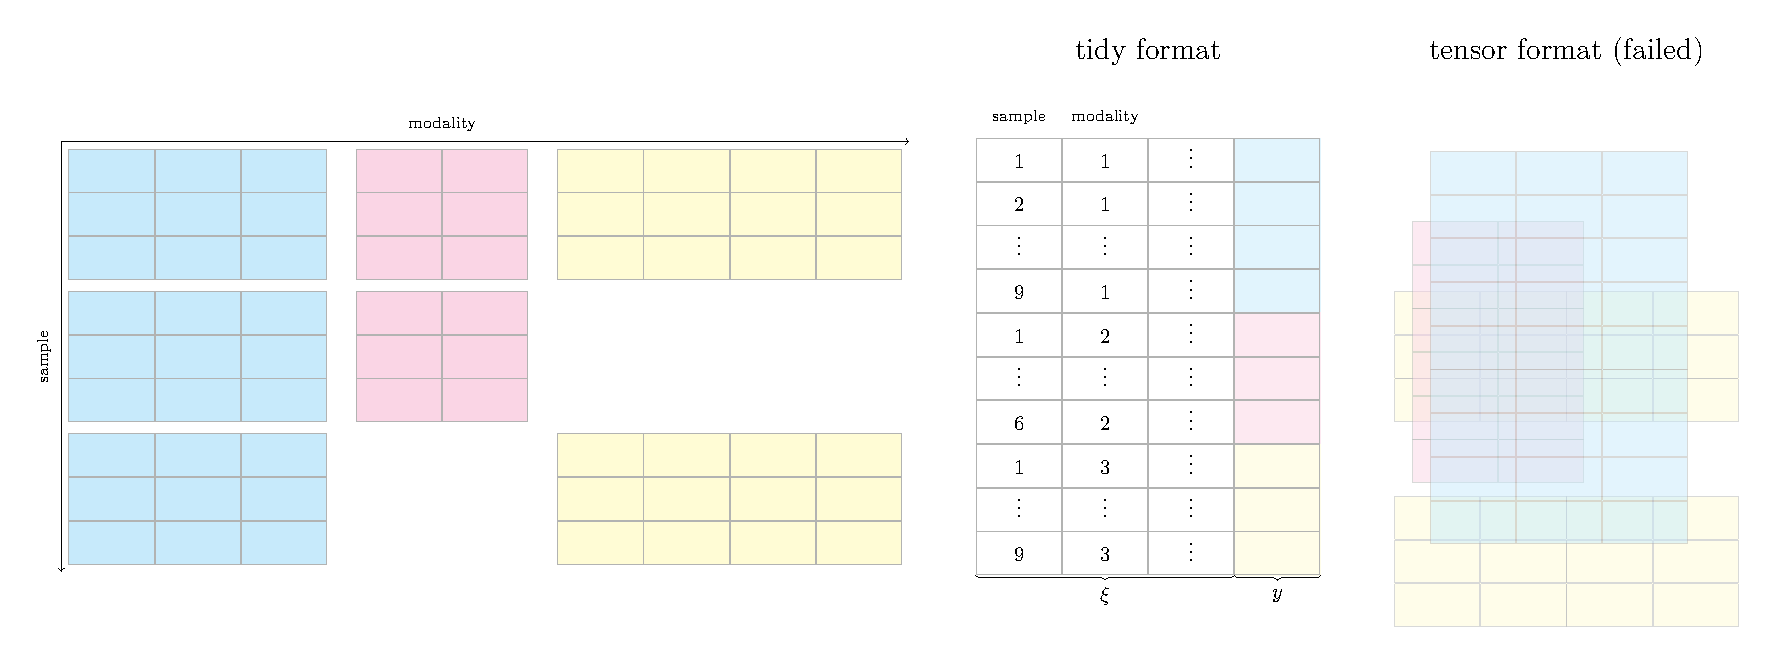
\includegraphics[width=0.95\textwidth]{img/mosaic}
\end{figure}
\begin{itemize}
\item semi-paired なデータが多い
\item モダリティごとに分布が変わる
\end{itemize}
}
\frame{


}
\end{document}  